A pesquisa proposta, assim como os temas abordados nela, é multidisciplinar. As próximas sessões abordarão tópicos necessários para o entendimento do projeto e suas abordagens.

Primeiramente será introduzido a linguística devido ao tema da análise de discurso, essencial para que seja possível analisar como as amostras se expressam em seus textos, além de uma introdução ao processamento de linguagem natural.

Em seguida, será necessário entender sobre Psicologia, dentro dela os tópicos traumas emocionais e modelos de mensuração que serão brevemente abordados devido ao cunho dessa pesquisa. Além disso, será introduzido ao conceito de Psicologia Cognitiva.

Os tópicos já explicados serão utilizados para dar fundamento a inteligência artificial. Nessa sessão também seram apresentados os conseitos básicos da área e o conceito de agentes. Em seguida será aprofundado o tema aprendizado de máquina, onde sera explicado conceitos e abordagens utilizadas por essa ramificação da IA.

Por fim, será tratado o tema \textit{data science}, os tópicos relacionados a manipulação de dados, desde a mineração e gestão até a sua representação e organização.

\section{Linguística}
A gramática é composta por: um conjunto finito de letras que formam o chamado alfabeto e um conjunto de regras e normas. Utilizando das regras e do finito número de palavras formadas a partir das letras, é possível se expressar através de uma sentença. O estado representado por essa sentença pode variar de acordo com a regra aplicada. É impossível cobrir todos os estados com uma única regra pelo motivo de existirem números infinitos de sentenças a serem formadas \cite[13-25]{chomsky2002syntactic}. Essa capacidade de obter descrições de forma simplificada através da linguagem é a primeira área cognitiva do ser humano \cite[131]{putnam1975mind}.

No dia-a-dia, existem multiplos fatores que ajudam a entender o sentido de uma frase, porém, em uma máquina os mesmos fatores muitas vezes não se aplicam. Nessa sessão o enfoque é em introduzir alguns estudos fomentados pela linguística. Na inteligência artificial, o ato de juntar símbolos (padrões físicos) em expressões (estruturas) utilizando um conjunto de regras (processos), é considerado um sistema de símbolos físicos. Acredita-se que um sistema desse formato possui os meios necessários e suficientes para realizar ações inteligentes de forma geral \cite[116]{newell1976ComputerSA}. Entretanto, o que foi escrito pode ser compreendido de forma diferente, vide duplo sentidos, isso torna o contexto extremamente relevante para o entendimento. Dentro da linguística existem estudos que permitem analisar o que foi redigido afim de entender o sentido que o autor quis transmitir.

% sections
\subsection{Análise de Discurso}
No decorrer de um texto (que é algo concreto), pode-se caracterizar diversos níveis de geração de sentido.
A primeira formulação de sentido vem do discernimento de termos dentro de um contexto, esse nível é chamado de fundamental. Após distinguir esse primeiro sentido ele é aplicado pelo autor através de um sujeito fazendo com que a prosa tome uma direção, esse nível é chamado narrativo. Por fim, existe o nível discursivo, relacionado as escolhas de tempo, espaço, pessoa e figura durante a narrativa dos fundamentos, dando a essa narrativa um ponto de vista. Logo, o termo discurso é dado como um suporte abstrato por trás do texto, afim da concretização da sua idéia central \cite[13-17]{gregolin1995ad}.

A análise de discurso é, de forma sucinta, uma análise do que foi dito, de como foi dito e qual o sentido do que foi dito. As primeiras manifestações do assunto foram no século XX com autores russos que, além de isolar e definir elementos de uma linguagem poética queriam definir determinantes por trás do perfil artístico do escritor. O tempo fez com que a análise de discurso se desenvolvese e ramificasse em várias vertentes, uma delas a francesa, que apoia a possibilidade de automatizar essa análise por meio da informática. A área continua sendo um campo complexo e de contínuo estudo por trás das definições e metodologias para abordar e sustentar as novas unidades de análise. \cite[22]{souza2006ad}.

Os discursos se diferem de pessoa para pessoa devido ao nível discursivo, a necessidade de expressar um determinado sentido leva o autor a se colocar em um ponto de vista durante sua narrativa. Do contexto da pesquisa, entender o discurso do usuário para mapear o motivo do seu estado mental é um fator de total relevância para entender o estado dele. A pesquisa realizada por Modesto Leite \cite[134]{modesto2005adepre}, mostra em seus resultados que os discursos apresentados pelos pacientes fundamentavam o motivo psicológico do por que os mesmo teriam o transtorno. 

Partindo dos principio apresentados sobre um discurso, por mais que as palavras sejam localizadas, o ponto chave da discussão está em como um computador seria capaz de inferir o sentido da frase. Existem áreas, seguindo os campos multidiciplinares que envolvem linguística e computação, responsáveis por garantir que o processamento dos textos gerará os resultados esperados.

\subsection{Processamento de Linguagem Natural}
Se entender palavras não significa entender o contexto, logo, se familiarizar com o ambiente e o momento afim de idealizar o que está sendo transmitido é algo necessário. Essa conexão entre elementos é tratada no estudo do \textit{connectivism}\footnote{Integração dos princípios de rede, caos, complexidade e teorias de auto-organização. Seu objetivo é entender decisões baseado nas mudanças de componentes fundamentais \cite{siemens2014connectivism}.}. De acordo com a linha de pensamento, estabelecida pelo estudo, os neurônios seriam os agentes cognitivos responsáveis por planejar, construir e representar essas informações que o cérebro humano recebe. Criar soluções para problemas pontuais que envolvam a língua que é utilizado no dia-a-dia de uma pessoa, essa é a definição por trás do Processamento de Linguagem Natural (PLN). Fornecer dados linguísticos que a maquina não é capaz de inferir, ou que seja necessário uma ajuda para seu melhor desempenho, é o ponto principal dessa área \cite{brandura1996, maria2015npl}.

Já que o PLN será inicialmente utilizado para análise de palavras-chaves e padrões, é necessário vislumbrar que será necessário um conjunto de regras a fim de melhorar uma determinada métrica durante o processo de aprendizagem. Para que isso seja possível, um conhecimento dentro da área de psicologia se torna altamente relevante.


\section{Psicologia}

A psicologia é descrita como a ciência da vida mental, capaz de entender o posicionamento e o estado emocional do ser, analisando os desejos, razões, sentimentos, decisões entre outras faculdades mentais. Esse entendimento de como o estado mental das pessoas impacta em sua vida é o grande desafio da área \cite[4-8]{william1890principles}.

A pesquisa utiliza da psicologia em dois pontos distintos. O primeiro deles é o envolvimento da psicologia com transtornos de humor, seguido da participação na área da psicologia cognitiva e seu impacto na evolução dos modelos computacionais. Existem vários transtornos de humor descritos pelo DSM-IV\footnote{É um manual famoso que auxilia no diagnóstico de desordens mentais\cite{dsmiv}}, entretanto, as suas causas são variadas. Entender o conceito de como alguns sentimentos impactam esses transtornos é fundamental nesse momento.

% sections
\subsection{Dimensões Afetivas Negativas}
Se caracteriza dimensão afetiva, também conhecida como afetividade, um conjunto de sentimentos que nos afetam positiva ou negativamente \cite[2-6]{pinto2009afetos}. Logo, quando abordado as negativas, pode-se pensar em tristeza, inveja e desesperança por exemplo, porém, o contexto da pesquisa será limitado as dimensões afetivas negativas: depressão, ansiedade e stress.

A depressão é uma forma atenuada de melancolia \cite{roudinesco2000psicanalise}, que por sua vez, seria uma condição maléfica de enfraquecimento da saúde mental de um ser. Classificada como transtorno de humor, a depressão, diferente de outras variações mais regulares de humor, pode causar grandes danos a vida cotidiana uma vez que, por definição, altera a percepção de si mesmo maximizando o peso dos seus problemas diante de sua própria perspectiva \cite{esteves2006depressao}. A melancolia e a depressão compartilham de sintomas em comum como: desânimo, perca de interesse, inibição, bloqueio de sentimentos e outros mais \cite[28]{freud2014livro}. No Brasil há uma média de 11 milhões de pessoas afetadas por esse transtorno \cite{paho2017-letstalk}, sem contar os demais transtornos correlacionados, a partir desses dados já se nota a importância do assunto e as propostas feitas para auxiliar no seu combate.

Existe também a ansiedade. Muitas das desordem relacionadas a ansiedade são categorizadas pelo medo e evasão do usuário a um assunto especifico \cite[393]{dsmiv}. Esse sentimento é primitivo e tem fortes semelhanças as reações animais de defesa ao se colocarem em um ambiente hostil. A inibição, assim como na depressão, é um dos sintomas dos transtornos relacionados a ansiedade, porém, o comportamento do ser usuário assume um formato mais similar a um excesso de vigilância e preocupação \cite{margis2003relaccao}.

Durante os estudos das dimensões afetivas negativas, algumas dificuldades em analisar casos de ansiedade e depressão foram encontradas. Com um menor impacto ao estado clinico, porém, podendo apresentar estados inicias dos outros dois transtornos, o agrupamento de sintomas composto por tensão, irritabilidade e dificuldades para relaxar foi denominado Stress. \cite{lovibond1995structure, ribeiro2004contribuiccao, margis2003relaccao}

Já estabelecidas as diferenças e relações entre a ansiedade, depressão e o stress, torna-se questionável como mensurar seu impacto em um ser humano. Essas dimensões foram selecionadas devido a existência de escalas já testadas para analisar e avaliar pacientes que as portem.



\subsection{Escala de Depressão, Ansiedade e Stress (EADS)}
Adotando um modelo dividido em três sub-escalas a Escala de Depressão, Ansiedade e Stress ou EADS foi proposta na premissa de uma maior assertividade na analise das dimensões afetivas negativas. Já existiam outras pesquisas com propostas similares como a Escala de Ansiedade de Beck e a Escala de Depressão de Beck. As diferenças entre essas escalas e a EADS são: a proposta de correlação entre os transtornos, a introdução de uma escala para o stress e a execução para obter os resultados partindo dessas novas abordagens.

A EADS completa é composta de 42 itens, para fins de facilitar a geração de dados será utilizado o modelo de 21 itens. Essa escala, como já foi citado, é dividida em três sub-escalas representando a depressão, ansiedade e stress. Essa divisão é simétrica, ou seja, cada sub-escala contém sete itens. O mais interessante é o fato, também ja abordado, da EADS propor uma correlação entre as dimensões, logo, um item pode pertencer a uma sub-escala, porém afetar uma segunda. Os itens dentro dessas sub-escalas são afirmações que podem ser respondidas por números de 1 á 4 e representam desde "não se aplica a mim" até "se aplicou a mim na maior parte das vezes". Representam as dimensões mais negativas os maiores valores gerados pela soma dos itens de cada sub-escala \cite{lovibond1995structure, ribeiro2004contribuiccao}.

Diferente da proposta de auto avaliação ou avaliação mediada\footnote{Nesses casos os usuários são responsáveis por responder as perguntas por si mesmos ou por meio de um mediador que ira preencher o formulário.}, como é proposta pela EADS,  um dos objetivos da pesquisa é inferir os resultados das escalas utilizando textos cotidianos de uma amostra coletada no Twitter. Isso nos leva a entender os conceitos cognitivos por trás da psicologia que levaram os autores a propor suas escalas e pesquisas.

\subsection{Psicologia Cognitiva}
Dentro da Psicologia existe um ramo cujo objetivo é entender a capacidade animal de pensar, memorizar, perceber e no caso humano utilizar um dialeto (linguagem), essa área de estudo ficou conhecida como psicologia cognitiva. \cite[3-9]{neisser2014cognitive}

O ato de entender os procedimentos cognitivos adotados pelo ser humano se tornou mais relevante após a proposta da criação de uma inteligência artificial. O questionamento de como uma decisão poderia gerar, afetar ou cancelar uma cadeia de eventos, seja ela durante um pensamento ou uma ação, partindo da capacidade humana de realizar múltiplas tarefas, algumas delas complexas como interpretar linguagens com tantas divergências, fez com que em 1958\cite[4-7]{broadbent1958perception} surgisse o primeiro modelo psicológico que propunha um fluxo similar ao processamento de informações de um computador.

As técnicas experimentais, como os modelos psicológicos, impactaram toda a área interdisciplinar das ciencias cognitivas. Novas abordagens como a junção de modelos criados em computação para IA e técnicas experimentais da psicologia foram criadas a fim do entendimento da mente humana. Durante a criação do \textit{General Problem Solver} ou em tradução literal Solucionador Geral de Problemas, por exemplo, Newell e Simon propuseram não só a implementação de algoritmos descritos por antigos estudiosos afim de resolver um série de problemas, mas também, entender como a máquina estava realizando isso, assim, seria possível uma comparação com a mente humana \cite{newell1961gps, russell2003artificial}.

Nessa pesquisa, a psicologia cognitiva terá um grande impacto em entender como as amostras que contem ou não sintomas causados pelas dimensões afetivas negativas se comportam e pensam. Esse entendimento é essencial para o mapeamento dos atributos que serão processados pela IA afim de gerar os modelos para predição em dados ainda não analisados. Além disso, a psicologia cognitiva faz parte de todo o processo qualitativo de criação, devido a ser um dos vários campos que compões a multidisciplinaridade dentro da IA.

\section{Inteligência Artificial}

Inteligência é, por definição, uma coleção sistemática de habilidades e funções com objetivo de processar diferentes tipos de informações de diversas maneiras \cite[49]{guilford1982cognitive}. Simular essa "coleção sistemática de habilidades e funções", reconhecer formatos, trajetórias, sinais, deduzir proposições entre outras, criando entidades inteligentes é o foco da inteligência artificial.

Do momento em que a IA passou a ser um campo de estudo em 1950, com as propostas de Turing, até o momento atual, a quantidade de abordagens apresentadas por diversos pesquisadores, afim de construir uma máquina inteligente apenas aumentou. Esses métodos se auto-contribuíram propondo novas visões e gerando novas abordagens a partir de descobertas dentro das suas linhas de pensamento. Isso levou a IA para seu estado atual. \cite[1-2]{russell2003artificial}.

No decorrer desta sessão serão apresentados os fundamentos visando introduzir as demais áreas que colaborarão com a computação para a criação da inteligência artificial, seguido pelas definições de agentes racionais.

\subsection{Fundamentos da Inteligencia Artificial}
Nas últimas sessões foram abordados os temas linguística e psicologia, e claramente é possível vislumbrar sua relevância dentro da área de Inteligência Artificial. A razão é o fato de ambas serem fundamentos da IA assim como outras áreas que serão dissertadas nessa sessão.

A engenharia da computação tem como foco construir máquinas eficientes, seja impactando com novos \textit{hardwares}, afetando diretamente o potencial de processamento e armazenamento das máquinas, ou com a criação de novos sistemas operacionais, linguagens e ferramentas que podem desde auxiliar na \textit{performance}, organização ou complexidade do problema até possibilitar criação de novas abordagens e implementações de algoritmos mais complexos. \cite[13-14]{russell2003artificial}.

Na busca de um melhor resultado durante a criação de um sistema inteligente, o processamento de dados é algo essencial. Em certos momentos os dados não fornecerão diretamente o que é necessário, e o ato de assimilar uma verdade baseado em outra verdade já conhecida, também chamado de inferência, já não será suficiente para gerar bons resultados, sendo assim, é necessário utilizar de recursos fundamentados e probabilísticos como equações matemáticas para resolver o problema. Para que isso se torne possível, será necessário extrair um dado exato de algo abstrato, por exemplo o \textit{sentistrength}, que retira o sentimento a partir de um trecho de texto \cite{boole1854investigation}.

Além dos conceitos de matemática, existem fatores da economia que fundamentam a IA. Diferente do que sugerido, essa área não se trata de dinheiro, mas de como é guiada as decisões baseadas nos retornos esperados. Os estudos da economia ainda aplicam-se a como agir perante expectativas de curto, médio ou longo prazo e se é viável continua-las quando outros fatores não estiverem favorecendo o ambiente \cite[9]{russell2003artificial}. Abordando o ambiente não só como o \textit{software} e sim como um mundo externo a ele, existe um fundamento, que não será aprofundado por não ter impacto nesta pesquisa, nomeado cibernética e a teoria de controle. Foi criado por Wiener\cite{wiener1961cybernetics} e visa o uso de componentes elétricos para coletar informações externas á máquina e traduzi-los para uma linguagem (numérica) na qual a máquina seja capaz de compreender.

Existem campos, como a própria linguística citada, que procuram sair da forma descritiva que atuam, propondo-se adotar modelos e definições exatas para guiar seus estudos. Esse foi o caso da neurociência, que é responsável por estudar o cérebro humano, ou seja, como as redes neurais funcionam \cite[10]{russell2003artificial}.

A biologia em si era em grande parte descritiva, embasada por anos de observação e pesquisas que até hoje apoiam suas definições. Sair desses padrões levou os cientistas a vislumbrarem a possibilidade de tratar o metabolismo como um centro de transmissão. Esse centro enviaria diversas transmissões que por sua vez emitiriam uma força. Essa afirmação levaria os cientistas a poderem calcular a força dessas transmissões afim de chegar em um modelo matemático plausível para replicar o funcionamento das redes neurais \cite[1-3]{rashevsky1960mathematical}. Entretanto, duvidas como até onde pode-se um computador suportar ou superar o processamento de um cérebro humano foram levantadas. Mesmo com tantas discussões em torno do assunto, a proposta de Vinge sobre uma super-máquina que superaria a inteligência humana, também chamada de singularidade tecnológica, continua não tendo uma comparação informativa atualmente, e mesmo que atualmente existisse a capacidade de ter-se memória e processamento infinito ainda não é possível entender como armazenar e replicar os padrões encontrados na neurociência \cite[11-12]{vinge1993coming,russell2003artificial}. Os estudos cognitivos tornaram possível entender melhor o funcionamento da mente humana. O método racional e a proposta de pensar nos meios que nos levam a um fim fez com que fosse capaz de abstrair modelos inteligentes através de agentes. A neurociência, por sua vez, forneceu a magnitude de como transmitir conhecimento e aprimorar os modelos, o fator inteligência e aprendizado passaram a ser mais vistos dentro do ramo de IA, nos levando a ascensão da aprendizagem de máquina.

Diferente das ciências onde existem fatos, teorias e pesquisas conclusivas, existem áreas capazes de fomentar intelectualmente assuntos diversos. O conceito de lógica, por exemplo, é algo relativamente descritível e aplicável aos conceitos da ciência, porém a teoria por trás do que viria ser lógico e o que faria um pensamento ser racional é algo muito mais complexo, em suma, o conceito de lógica já era debatido por estudiosos na Grécia antiga. A filosofia tem sua relevância pra IA pois contribuiu com ideias como o \textit{Law of thought} (lei do pensamento), que em contra partida ao pensar humano, é uma lei psicológica que acompanha um processo mental, logo, necessita estar de acordo com uma razão ou lógica \cite{frege1956thought, russell2003artificial}. Além disso, a filosofia foi responsável por estudos como o racionalismo onde é dito que é possível adquirir conhecimento independente da experiência sensorial. Originada dessa ideia nasceram o dualismo, onde é afirmado que a mente é algo natural e sem conhecimento do mundo externo, e o materialismo, que contrariando o dualismo afirma que a mente é formada pelas operações do cérebro. Em negativa ao racionalismo, existe o empirismo, onde é definido que a experiência sensorial é a fonte final de conhecimento \cite[6]{rationalismvsempiricism, descartes2013rene, russell2003artificial}. Estes estudos tiveram sua relevância sobre o pensamento racional e como seria possível criar máquinas que pensassem e agissem racionalmente.

\subsection{Agentes Racionais}
“Mas seria possível uma máquina pensar?“ Esse questionamento inicial de Turing, desencadeou a proposta do \textit{Imitation Game}, que basicamente consiste em colocar uma pessoa (1) para conversar com um computador, esse computador poderá ser uma inteligência artificial ou outra pessoa (2) conversando através da máquina. O objetivo é que a pessoa 1 consiga distinguir se quem esta conversando com ela é a máquina ou a pessoa 2. A proposta feita por Turing seria considerada como um agir humanamente. Ela baseia-se em criar uma máquina que reconhece a escrita, tome decisões a partir de um base de dados e por final seja capaz de se aprimorar diante de novos cenários. Porém, como seria desenvolvido algo de tal amplitude? A resposta é que “não seria”! Questionar se uma máquina é capaz de pensar seria o mesmo que questionar se um submarino é capaz de nadar, afirmou Dijsktra, apontando que o termo "pensar" e "nadar" tinham suas definições restritas, entretanto, era possível realizar ações similares tão bem quanto \cite[2-3]{dijkstra898, turing1950, russell2003artificial}.

Para realizar as ações descritas por Turing, é necessário entender os passos descritos por ele de forma racional e lógica afim de replicá-los para a máquina.

A abordagem de agentes racionais é uma das possibilidades a serem usadas. O termo racional significa algo baseado ou acordado com uma razão ou lógica, de outro lado, a lógica tem dois pilares: a conversão responsável por expressar a mesma proposição em diferentes formas e o silogismo responsável por localizar um termo em comum que conecte duas dessas proposições. Um agente é algo que age, ou seja, um agente racional seria quem analisa circustâncias utilizando de definições lógicas e racionais a fim de interagir com algo. Isso é afirmado pela definiçao de Russel\cite[7]{russell2003artificial}, onde um agente racional percebe modificações no ambiente, através de sensores, e interage de volta com o ele novamente através de atuadores. Pode-se notar esse fluxo na Figura \ref{fig:rational_agent_draw}.

Logo, é possivel afirmar, que para ser possível realizar ações racionais é necessário entender o ambiente aonde você esta e suas variáveis, alias, é necessário que esteja claro o que pode ou não ser computado, quais são as regras que se aplicam e principalmente como obter algo racional com base em informações abstratas ou com dados incompletos \cite{frege1956thought, wooldridge1994agent, simon1955behavioral, boole1854investigation, russell2003artificial}

\begin{figure}
    \centering
    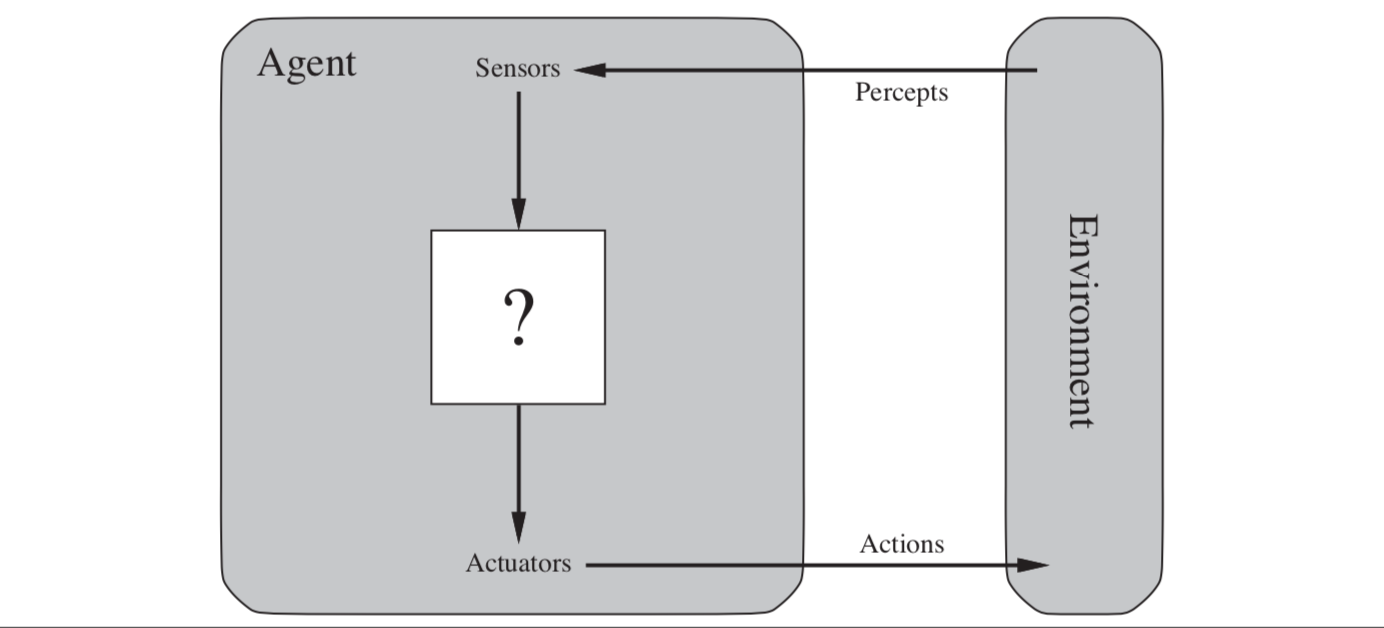
\includegraphics[width=.8\textwidth]{imagens/rational_agent_draw.png}
    \caption{Fluxo executado por um agente racional. Fonte: Russel, 2003, 35. Adaptada pelo Autor}
    \label{fig:rational_agent_draw}
\end{figure}

Definir se o agente está ou não gerando os dados esperados é um dos passos durante o desenvolvimento dos agentes. É necessário analisar o ambiente gerado a partir das percepções e conferir se os dados são os esperados ou não, essa etapa chama-se mensuração de \textit{performance}. Resumidamente, o agente receberá um entrada de dados e será responsável por gerar um saída. Ao longo do tempo o mesmo agente gerara múltiplas percepções e essas formarão uma sequencia de percepções \footnote{Não serão todos os modelos que seguirão a proposta sequencial, existem casos em que a linha temporal não afeta o desenvolvimento da decisões tornando-as episódicas}.

Existem vários tipos de agentes racionais, sendo definidos como \cite[34-45]{russell2003artificial}:

\begin{itemize}
 \item Totalmente, parcialmente ou não observador: essa definição é gerada pela quantidade de fatores do ambiente que seu agente recebe, um agente que tem todas as informações do ambiente é totalmente observador enquanto um que não recebe nada, precisando assim manter alguns estados, é não observador.
 \item Estocástico ou Determinístico: quando é impossível determinar o próximo estado através do anterior o agente é Estocástico, caso ao contrario ele é Determinístico.
 \item Episódicos ou Sequenciais: já foi dito que em diversas abordagens são gerados sequencias de percepção, quando essa sequencia é alterada a partir de alguma mudança de estado o agente é chamado de sequencial, caso ao contrario o agente é episódico.
 \item Estáticos ou Dinâmicos essa definição é referente ao ambiente, quando o ambiente não infere alterações o agente é nomeado estático, caso ao contrario Dinâmico.
 \item Continuo ou Distinto: Quando existem finitas possibilidades de estado pode se afirmar que o agente é Distinto, quando as possibilidades são infinitas é dado o nome de Continuo.
 \item Conhecido ou Desconhecido: Quando o agente necessita aprender algo e não consegue realizar a ação por si só ele é um agente desconhecido, caso contrário ele é conhecido.
\end{itemize}

Porém, é necessário diferenciar um agente racional de um algoritmo de tomada de decisão. O fato é que um agente pode tomar uma decisão, porém ele não gera só uma solução, mas sim, a equação necessária para conseguir essa solução. Além disso, baseado em um sistema inteligente com múltiplos agentes racionais, fica-se o questionamento sobre o quão inteligente um agente isolado pode ser, e também, quantos agente são necessários para que a máquina consiga obter o conhecimento desejado. Essas questões levam a IA para o próximo passo: ensinar um sistema a coletar esses resultados.


\section{Aprendizado de Máquina}
Se máquinas pensam ou não, o enfoque da IA é executar diretamente um processo que um ser humano aprendeu ao longo dos anos, e não, algo que implicitamente nasceu com ele. Logo, o fluxo mais sistemático para conseguir que uma máquina abstrai formalmente um conhecimento seria mapear um estado inicial, aplicar dados para sua aprendizagem e submete-la a outras experiências afim de reafirmar esses conhecimentos. Essa abordagem foi proposta por Turing em 1950, entretanto, o campo de pesquisa conhecido como \textit{machine learning} ou aprendizado de máquina surgiu, apenas em 1959 quando o termo nasceu ao ser aplicado em um estudo de redes neurais. Portanto, pode-se brevemente descrever o aprendizado de máquina como métodos computacionais designados a utilizarem de algoritmos precisos de predição juntamente a uma base de conhecimento para aumentar a sua assertividade\cite[1]{turing1950, samuel1959some, mohri2012foundations}.

Nessa sessão é dado um enfoque maior em \textit{machine learning}. Primeiramente serão introduzidos alguns conceitos que são utilizados a partir dessa sessão. Com os conceitos passados, sera apresentado, de maneira lacônica, a aplicação dos conceitos perante algoritmos de aprendizado de máquina. Por fim, é sugerido algumas ferramentas utilizadas para implementação do \textit{machine learning} e um breve enfoque em como é guiado esse campo dentro desta pesquisa.

\subsection{Conceitos do Aprendizado de Máquina}
Previamente foi dito que, seriam necessários dados de treino, esse dado bruto, como já dito também, contém várias propriedades que podem ser ou não processadas afim de gerar informações, esse dado é conhecido com dados de treinamento e um dado que contém as informações processadas necessárias, inserida por algoritmos ou por fatores externos, é chamado de dado rotulado ou anotado.

As propriedades podem ser utilizadas para classificar um determinado dado, isso as concede o nome de atributo. Também conhecido com \textit{feature}, é considerada como um dos fatores mais relevantes para o aprendizado da máquina. O termo conhecido como \textit{feature engineering} ou, em tradução literal, engenharia de atributos, diferente do processo de aprendizagem em si, são baseados diretamente a suas entidades e em como escolher e pré-processar seus atributos chaves afim de otimizar o aprendizado \cite{domingos2012few}.

Esses atributos, dentre outras propriedades, estão em uma massa de dados. Por sua vez serão utilizadas como dados de entrada para um agente. Esse agente também pode ser representado, por fins explicativos, como uma simples função \textit{f(x) = y}, o objetivo é treinar o agente para que ele seja capaz de generalizar. Ou seja, capaz de predizer o melhor valor para \textit{y} a partir da entrada \textit{x}. Quando o resultado final depende totalmente dos dados de entrada, ou seja, não existem muitas variações que levem a saída a grandes divergências, é dito que o problema generaliza bem.

Essa função gerada que sucintamente traduz os padrões encontrados entre os dados, gera um modelo. Muitos deles são utilizados para classificar os dados dentro de um grupo de possibilidades, esse tipo de modelo é descrito como classificador.

Os problemas a serem processados pelos classificadores ou outros modelos possuem um conjunto de  hipóteses. Quando é concebida uma preferência a uma dessas hipóteses com a premissa de induzir o modelo a tomar uma decisão é dado o nome de tendência.

Uma quantidade extensa de hipóteses e dados de entrada não significam uma máquina mais assertiva. Quando um agente é treinado para executar mais do que o necessário, um fenômeno peculiar chamado de \textit{overfitting} ou sobre-ajustes acontece, esse evento faz com que a máquina seja capaz de tomar decisões assertivas apenas para um conjunto de dados a qual foi submetida e não consegue predizer novas entradas.

As descrições dadas por Russel \cite[693]{russell2003artificial} ainda se aplicam a conceitos mais complexos que não cabem a essa pesquisa explicitamente. O jeito que são utilizados os dados ou os atributos previamente ditos, podem resultar em diversos tipos de abordagens diferentes essas abordagens são conhecidas por diversas categorias de algoritmos que podem ser implementados para solucionar um problema.

\subsection{Métodos de Aprendizagem}
Os atributos presentes nos dados podem ser utilizados com a premissa de predizer uma determinada hipótese. A aprendizagem supervisionada, como pode-se observar na figura \ref{fig:supervisedlearning}, justifica-se por separar o conjunto de dados em duas bases: teste e treinamento, posteriormente, utilizar as bases para produzir um modelo de predição capaz de satisfazer uma hipótese. Usualmente dentro da aprendizagem supervisionada existe um método que consiste em utilizar de um atributo discreto ou qualitativo e a partir de um indutor gerar o melhor classificador para aquele problema, esse método é chamado classificação. Ainda existe um outro, que se baseia em atributos contínuos, com isso é possível utilizar de predição numérica afim de identificar um modelo dentro do plano cartesiano e prever futuros valores para o mesmo atributo em outras situações, esse método se chama regressão. \cite{hastie2009unsupervised, russell2003artificial}

\begin{figure}[!h]
    \centering
    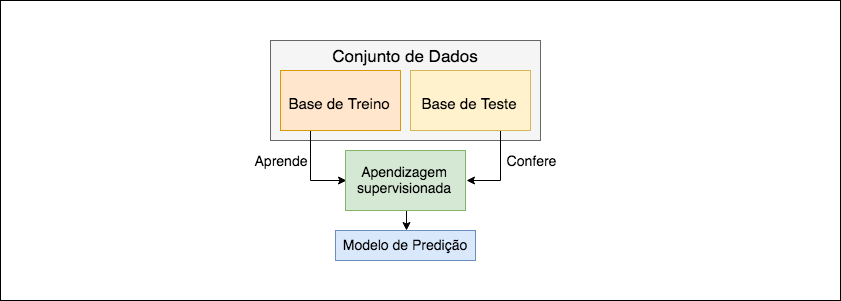
\includegraphics[width=.8\textwidth]{imagens/supervisedlearning.png}
    \caption{Diagrama representando os eventos da aprendizagem supervisionada.}
    \label{fig:supervisedlearning}
\end{figure}

Em contrapartida, existem casos onde os atributos não estarão anotados e a máquina terá que literalmente inferir a probabilidade em toda a base. Esse estilo de aprendizagem se chama aprendizagem não-supervisionada, e o enfoque é utilizar da segregação dos atributos e suas dimensões para inferir resultados. O método mais comum dentro desse estilo é a clusterização que, exemplificado na Figura \ref{fig:unsupervised}, se baseia em particionar os dados em grupos dentro de um plano cartesiano tomando de referência um ou mais atributos. Outra pratica utilizada nesse tipo de aprendizagem é redução dimensional, onde resume-se o estado atual de um item para um estado de menor complexidade de dimensões com base nas propriedades chaves \cite{hastie2009unsupervised, mohri2012foundations}.

\begin{figure}[!h]
    \centering
    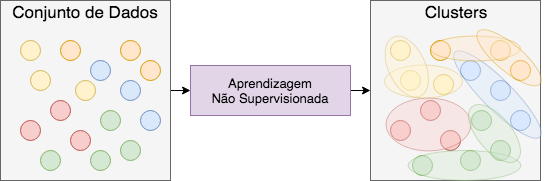
\includegraphics[width=.8\textwidth]{imagens/unsupervised.png}
    \caption{Diagrama representando a clusterização.}
    \label{fig:unsupervised}
\end{figure}

Ainda correlacionado com as últimas explicações, existe um tipo onde é inserido no agente dados anotados e não anotados para predição de todos os itens da base. A aprendizagem semi-supervisionada, suscintamente definida, é a mescla das duas outras aprendizagens. Utiliza da parte anotada (supervisionada) e da lógica de grupos (não-supervisionada), para normalizar e otimizar o resultado final \cite[7]{mohri2012foundations}.

Por último, existem casos onde não teremos dados suficientes para executar outros tipos de aprendizagem, nesse momento a aprendizagem é baseada na tradicional tentativa e erro. Nomeada aprendizado por reforço, ao observar a Figura \ref{fig:reinforcement} pode-se notar que se, consiste em um ambiente (A), responsável por emitir um estado para o componente, feito isso é aplicado uma entrada de dados (e) ao agente (G) que será responsável por tomar a decisão de que ação (a) tomará para a entrada (e) previamente recebida. Essa ação modifica o estado do ambiente e transmite um sinal de reforço visando através do componente (r) para que a aplicação tome a melhor escolha ao longo prazo \cite{kaelbling1996reinforcement, russell2003artificial}.

\begin{figure}[!h]
    \centering
    \scalebox{.5}{
\includegraphics[width=.8\textwidth]{imagens/reinforcement.png}}
    \caption{Diagrama apresentando o modelo sequencia ocorrido durante a aprendizagem por reforço.}
    \label{fig:reinforcement}
\end{figure}

Indiferente do tipo ou situação em que o algoritmo se enquadra, a multiplicidade de escolhas propostas pelo \textit{machine learning} gerou várias propostas de aprendizado, algumas até tentando utilizar da estrutura proposta pela neurociência para replicar nas redes neurais.

\subsection{Algoritmos de \textit{Machine Learning}}
É essencial entender que existem vários algoritmos de aprendizagem, para todos os tipos já apresentados durante esse referencial. Entretanto, será salientado alguns deles.

Um dos algoritmos é o \textit{support vector machine} ou SVM. Ele consiste em construir o máximo de separação entre os pontos, os vetores do SVN possibilitam que, por mais que o algoritmo trabalhe muito bem linearmente, ele crie separações em maiores dimensões. Por ultimo, sua maior vantagem é a flexibilidade, SVN pode suportar funções complexas, porem, é totalmente resistente ao sobre ajustes \cite[744]{russell2003artificial}.

Diferente de traçar vetores afim de estabelecer funções, existem métodos baseados em sequenciar varias unidades de processamento (similares aos agentes), afim de propagar uma entrada de dados e processá-la N vezes, por N fórmulas diferentes, afim de encontrar o melhor modelo possível a partir do dado de saída. Basear-se em camadas de unidade de processamento com a proposta de simular o comportamento do cérebro humano ao processar uma informação utilizando camadas de neurônios, essas unidades são fortemente coligadas uma vez que, todas as unidades de todas as camadas são obrigatoriamente interligadas. Essa abordagem ficou conhecida como redes neurais ou \textit{Neural Network} \cite{haykin2004comprehensive, russell2003artificial}.

Motivo de retorno dos estudos as Redes Neurais, e também um dos fatores que podem ser custosos para essa abordagem, é o \textit{back-propagation} ou retro-propagação é o termo utilizado para classificar o ato de ajustar os parâmetros de entrada da sua rede a partir dos dados de saída. Esse ajuste é feito de forma automatizada pelo próprio sistema afim de tentar igualar o valor de saída ao valor esperado. Quando uma rede neural apresenta muitas camadas ela passa a ser considerada uma estrutura de profundidade. Infelizmente, a retro-propagação não funciona muito bem para redes neurais com muitas camadas. Uma alternativa para isso, seria que nem todos os neurônios fosse interligados, e que os dados fossem reduzidos por necessidades isoladas se tornando cada vez mais específicos afim de que no final propor um conjunto de saídas para parâmetros esperados, essa abordagem ficou conhecida como \textit{Deep Learning} \cite{lecun2015deep}.

Independente da abordagem escolhida, é necessário um conjunto de dados para treinar sua máquina. Portanto, a extração desses dados e posteriormente sua manipulação, exploração e tratamento são essenciais para o sucesso da IA e dos resultados gerados por ela.

\section{Ciência por trás dos dados}
Como um ser humano, os dados têm seu ciclo de vida, esse ciclo pode alterar-se dependendo de sua finalidade dentro da aplicação. O tema e o objetivo desta pesquisa é coberto por uma matéria, já antiga, nomeada KDD ou \textit{Knowledge Discovery in Database}, como o próprio nome traduzido sugere, a Descoberta de Conhecimento em Base de Dados abrange varias subclasses como mineração de dados, analise de dados, probabilidade e até mesmo a própria IA. A KDD se justifica pela sua metodologia de manipulação de dados afim de extrair o conhecimento almejado de um base. Se observar o fluxo descrito na Figura \ref{fig:kdd}, pode-se notar que uma cadeia de eventos como: seleção, pré-processamento, mutação, mineração e interpretação. Esses eventos geram novos estados para o dado, e os moldam focando o objetivo de retirar o conhecimento pela interpretação no final do processo.

\begin{figure}
    \centering
    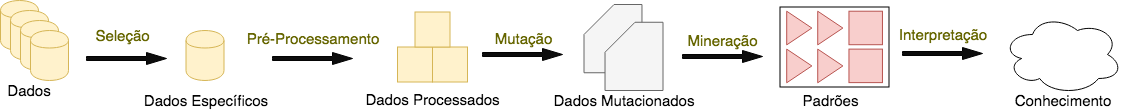
\includegraphics[width=.8\textwidth]{imagens/kdd.png}
    \caption{Representação da metodologia defendida pela KDD. Fonte: o autor.}
    \label{fig:kdd}
\end{figure}

Com o passar do tempo, várias abordagens surgiram para tratar dados e essa massa de pesquisas e definições deu-se por bagunçar em partes as nomenclaturas e definições que estão atrelados a ciência por trás dos dados. Para evitar confusões as definições apresentadas nessa sessão serão sucintas e tem como objetivo futuros tópicos e discussões apresentados durante os resultados dessa pesquisa. Devido a grande divergência, ocorrida pela disseminação rápida de algumas termologias, os termos abordados serão guiados pelas seguintes referencias \cite{laender2002brief, fayyad1996kdd, hand2007principles}.

\subsection{Coleta de Dados}
A coleta, é o ato de obter dados em massa de fontes externas, como \textit{websites} e \textit{apis}\footnote{A sigla API vem de \textit{Application Programming Interface} e é uma interface que permite outras aplicações utilizarem de seus recursos e funcionalidades. Dentro do universo \textit{web}, o termo API é utilizado para descrever um conjunto de rotas que podem ser utilizados para acessar recursos de um aplicação online.}. Também conhecido como \textit{data collection}, durante o processo do KDD é o primeiro passo responsável por gerar um amostra mais focada no problema.

No projeto será utilizada a API do Twitter para coletadar os dados para uso da aplicação. Durante a coleta é necessário entender as limitações da fonte de dados. No caso das API's é usual existir \textit{Rate Limits}, ou seja, limites de requisições, no caso do Twitter existem planos que aumentam ou diminuem seu acesso a API, no caso do projeto será utilizado a versão \textit{Standard} que é a versão gratuita para desenvolvedores\footnote{\url{https://developer.twitter.com/en/docs/basics/rate-limits.html}}. Alguns dos \textit{endpoints}\footnote{Um endpoint é uma URL acessivel por protocolos HTTP ou HTTPS e que retornam dados ou realizam ações} que serão:
\begin{itemize}
    \item \textit{users/show}: Responsável por pegar as informações do usuário, tem um limite de 60 requisições por minuto.
    \item \textit{statuses/user\_timeline}: Responsável por pegar os últimos tweets do usuário, tem um limite de 100 requisições por minuto.
\end{itemize}

Existe no projeto também, e recorrente em outros tipos de APIs, os \textit{streamings}, ou seja, recursos que serão consumidos através de uma requisição que fica aberta por tempo indeterminado recebendo novos dados.
\begin{itemize}
    \item \textit{statuses/filter}: Responsável por pegar os últimos tweets publicados por filtros. Na documentação será detalhado os filtros que serão utilizados na pesquisa, mas basicamente aqui é possível escutar as ultimas publicações feitas em escala global e coletar apenas as que compatíveis com um conjunto de filtros. Esse tipo de recurso não tem seu limite estabelecido por requisições e sim pelo seu uso (tentativas de reconexões por exemplo).
\end{itemize}

Uma vez coletados, outras ações descritas na Figura \ref{fig:kdd} como Pré-Processamento e Mutação serão realizados no próprio coletor enquanto outras serão realizadas posteriormente por \textit{scripts} e/ou ferramentas. A preparação do dado é relevante para assegurar a qualidade da mineração. No Twitter pode-se encontrar diversos problemas na hora da análise. Alguns dos mais populares são: A quantidade de ruído apresentado nos dados por erros de ortográfica, os uso de símbolos especiais como \textit{emojis} ou a inserção \textit{urls} ao longo do texto e por final a informalidade e contexto multilíngue, ou seja, o ato de escrever-se utilizando palavras fora do nosso idioma ou gírias pra manifestar algo. Além disso existe o fato de alguns processamentos, como a análise de sentimento, ter alguns problemas em textos muito curtos ou muito compridos. Pesquisas de 2012\footnote{\url{https://thenextweb.com/twitter/2012/01/07/interesting-fact-most-tweets-posted-are-approximately-30-characters-long/}}, demonstram que um tweet contém em média apenas 30 caracteres com o seu limite máximo, já pequeno, de 140 carácteres. \cite[9-11]{silva2016analise} Entretanto, no dia 27 de setembro de 2017, o Twitter anunciou\footnote{\url{https://blog.twitter.com/official/en_us/topics/product/2017/Giving-you-more-characters-to-express-yourself.html}} a expansão do limite máximo para 280 caracteres, o que abre possibilidade de textos mais pontuais na massa de dados coletada.

Uma vez conhecida as limitações e problemas da fonte de coleta, é possível idealizar e implementar soluções para contornar e/ou utilizar alguns recursos apresentados problemáticos.

\subsection{Mineração de Dados}
A mineração é um passo que ocorre após os dados terem sido devidamente normalizados. Vale ressaltar que para obter conhecimento não é necessário uma IA, sistemas de tomada de decisão trabalham com probabilidade matemática sob dados exatos, o que em muitos casos, já seria o suficiente para obter a informação do dado. Entretanto, o foco da pesquisa se baseia na implementação de um sistema inteligente e isso inclina essa explicação para o fato de: o aprendizado de máquina é uma das possíveis formas de se minerar um dado.

A mineração de dados ou popularmente conhecida como \textit{data mining}, baseia-se em retirar os valores mais relevantes e valiosos para se inferir um conhecimento. Os demais passos como pré-processamento e mutação se assemelham a alguns processos citados anteriormente como a redução dimensional ou ainda a engenharia de atributos.

No caso dessa pesquisa, a inferência de uma EADS baseada nas publicações de um usuário seria um tipo de dado extraído a partir de um modelo inteligente treinado por uma base de dados pré-processada. A caracterização de um perfil baseado em seus atributos, incluindo o próprio valor da EADS inferido, seria um outro exemplo do uso de IA para minerar a probabilidade de existir um certo nível de uma ou mais dimensão afetiva baseada em informações pessoais como sexo, localidade, trabalho e gostos pessoais.

Existem pesquisas voltadas a identificação de depressão dentro do Twitter, alguns dos atributos estabelecidos por eles como frequencia de postagem, a hora de maior atividade na rede social, sua interação com demais usuarios e até o óbvio uso de nome de antedepressivos nas frases, são taxados como ótimos atributos durante a mineração. \cite{de2013social, de2013predicting, tsugawa2015recognizing, yang2015gis}.

Com os dados em mãos, é possível, baseado no conhecimento fornecido pelo dado, realizar vários tipos de análise. O enfoque desse trabalho não é realizar hipóteses ou explorar os dados gerados, e sim, certificar a possibilidade da criação dessa base e a assertividade dos modelos, garantindo, que outros pesquisadores possam utilizar da base gerada nesse trabalho para realizar futuras pesquisas. Mesmo assim se torna relevante citar, mesmo que brevemente, a última parte do ciclo de um dado referente a consumir o conhecimento fornecido pelo mesmo.

\subsection{Análise de Dados}
O passo descrito como interpretação no KDD se refere a entender os dados de saída vindos da mineração afim de afirmar ou descartar hipóteses, com isso é possível refinar o processo e/ou explorar novas possibilidades. Existem 3 fortes termos quando tratamos a analise de dados:
\begin{itemize}
    \item - \textit{Data Exploration}: O ato de explorar os dados (conhecimento) gerados afim de localizar pontos relevantes e elaborar ou embasar hipóteses.
    \item - \textit{Data Storytelling}: O ato do dado contar uma história. Abordar a hipótese de maneira empírica e demonstrar a veracidade dela discutindo abordagem e algoritmos gerados é um dos objetivos dessa área.
    \item - \textit{Data Visualization}: O ato de demonstrar o dado através de representações gráficas ou tabelas, normalmente utilizados para embasar e demonstrar dados durante o \textit{Storytelling}.
\end{itemize}

Todos os conceitos apresentados acima, utilizados em conjunto ou separado, são parte necessária do processo de IA. Durante a pesquisa serão utilizados tais recursos com a premissa de refinar nosso processo de mineração/aprendizado, como demonstrar alguns dados gerados pela pesquisa.

